\documentclass[12pt]{article}
\setlength{\headheight}{24pt}
\usepackage[top=1.5in, bottom=1in, left=0.5in, right=0.5in]{geometry}
\usepackage{fancyhdr}
\usepackage{graphicx}
\usepackage{amsmath}
\usepackage{mwe} % for blindtext and example-image-a in example
\usepackage{wrapfig}
\usepackage{url}
\graphicspath{{./LoveAiri/Downloads/}}
\begin{document}
\fancypagestyle{firstpage}{%
  \lhead{\textit{\textbf{Name: Lai Man Hin}}}
  \chead{\textit{\textbf{SID: 1155136167}}}
  \rhead{\textit{\textbf{CSCI3230 Assignment 3}}}
}
\thispagestyle{firstpage}
CSCI3230 / ESTR3108 2021-22 First Term Assignment 3\\
I declare that the assignment here submitted is original except for source material explicitly acknowledged, and that the same or closely related material has not been previously submitted for another course. I also acknowledge that I am aware of University policy and regulations on honesty in academic work, and
of the disciplinary guidelines and procedures applicable to breaches of such policy and regulations, as contained in the following websites.\\
University Guideline on Academic Honesty:\\
\url{http://www.cuhk.edu.hk/policy/academichonesty/}\\
Faculty of Engineering Guidelines to Academic Honesty:\\
\url{http://www.erg.cuhk.edu.hk/erg-intra/upload/documents/ENGG_Discipline.pdf}\\
Student Name: \textit{\textbf{Lai Man Hin}}\\
Student ID : \textit{\textbf{1155136167}}\\
\textbf{1a)}\\
\begin{align*}
XX^{T} &= \begin{bmatrix}
1 & 0 & 1 & 0\\
1 & 0 & 1 & 0\\
1 & 0 & 1 & 0\\
\end{bmatrix}
\begin{bmatrix}
1 & 1 & 1\\
0 & 0 & 0\\
1 & 1 & 1\\
0 & 0 & 0\\
\end{bmatrix}
\\&= \begin{bmatrix}
2 & 2 & 2\\
2 & 2 & 2\\
2 & 2 & 2\\
\end{bmatrix}
\end{align*}
To find $XX^{T}$'s eigenvalue, we start at $|XX^{T} - \lambda I| = 0$\\
\begin{align*}
|XX^{T} - \lambda I| &= 0\\
\begin{vmatrix}
2-\lambda & 2 & 2\\
2 & 2-\lambda & 2\\
2 & 2 & 2-\lambda\\
\end{vmatrix} &= 0\\
-\lambda^{3} + 6\lambda^{2} - 12\lambda + 8 + 8 + 8 - 8 + 4\lambda - 8 + 4\lambda - 8 + 4\lambda &= 0\\
-\lambda^{3} + 6\lambda^{2} &= 0\\
\lambda &= 0 \text{ (double root) or } 6\\ 
\end{align*}
\newpage
\newgeometry{top=0.5in, bottom=1in, left=0.5in, right=0.5in}
\textbf{1b)}\\
To find the first principal axis of $X$, we should find the eigenvectors associated with largest eigenvalue (i.e. $\lambda = 6$)\\
Therefore,\\
\begin{align*}
\begin{bmatrix}
2 & 2 & 2\\
2 & 2 & 2\\
2 & 2 & 2\\
\end{bmatrix} \begin{bmatrix}
v_{1}\\
v_{2}\\
v_{3}\\
\end{bmatrix} &= 6 \begin{bmatrix}
v_{1}\\
v_{2}\\
v_{3}\\
\end{bmatrix}\\
\end{align*}\\
Then, we have
\begin{align*}
\begin{cases}
2v_{1} + 2v_{2} + 2v_{3} = 6v_{1} & (1)\\
2v_{1} + 2v_{2} + 2v_{3} = 6v_{2} & (2)\\
2v_{1} + 2v_{2} + 2v_{3} = 6v_{3} & (3)\\
\end{cases}
\end{align*}\\
By considering $v_{1} = v_{2} = v_{3}$, we have
\begin{align*}
\begin{cases}
6v_{1} = 6v_{1}\\
6v_{2} = 6v_{2}\\
6v_{3} = 6v_{3}\\
\end{cases}\\
v_{1} = k, v_{2} = k,  v_{3} = k  \indent (k \neq 0)\\
(\text{e.g.   } v_{1} = 1, v_{2} = 1,  v_{3} = 1)\\
\end{align*}
So, we have $\begin{bmatrix}
1 \\ 1 \\ 1
\end{bmatrix}$ as the first principal axis, the first principal component is given by\\
\begin{align*}
U^{*T}X &= \begin{bmatrix}
1 & 1 & 1\\
\end{bmatrix}
\begin{bmatrix}
1 & 0 & 1 & 0\\
1 & 0 & 1 & 0\\
1 & 0 & 1 & 0\\
\end{bmatrix}\\
&= \begin{bmatrix}
3 & 0 & 3 & 0\\
\end{bmatrix}
\end{align*}\newpage
\textbf{1c)}\\
They should be identical by discovering the new $XX^{T}$,\\
\begin{align*}
XX^{T} &=
\begin{bmatrix}
1 & 0 & 0 & 1\\
1 & 0 & 0 & 1\\
1 & 0 & 0 & 1\\
\end{bmatrix}
\begin{bmatrix}
1 & 1 & 1\\
0 & 0 & 0\\
0 & 0 & 0\\
1 & 1 & 1\\
\end{bmatrix}\\
&= \begin{bmatrix}
2 & 2 & 2\\
2 & 2 & 2\\
2 & 2 & 2\\
\end{bmatrix}\\
\end{align*}
We get the same answer as (a), so we will have the same principal axis, ($\begin{bmatrix}
1\\1\\1
\end{bmatrix}$). 
No matter how the columns exchange, it will still have the same principal axis. Therefore, it is proven that the order of input record will not affect the resulting principal axis we want to obtain.\\[0.5in]
\textbf{2a)}\\
Let $g(\mu) = (X^{(i)} - \mu ) - UU^{T}(X^{(i)} - \mu )$, so\\
\begin{align*}
\dfrac{\partial g(\mu)}{\partial \mu} = -I + UU^{T}
\end{align*}
Using the chain rule in L2 norm,
\begin{align*}
\dfrac{\partial f(\mu)}{\partial \mu} &= \sum_{i=1}^{m}2(\dfrac{\partial g(\mu)}{\partial \mu})^{T}g(\mu)\\
&= \sum_{i=1}^{m}2(-I + UU^{T})^{T}((X^{(i)} - \mu ) - UU^{T}(X^{(i)} - \mu ))\\
&= \sum_{i=1}^{m}2(-I + UU^{T})((X^{(i)} - \mu ) - UU^{T}(X^{(i)} - \mu ))
\end{align*}\\
\textbf{2b)}\\
\begin{align*}
\dfrac{\partial^{2}f(\mu)}{\partial \mu^{2}} &= \sum_{i=1}^{m} 2(-I + UU^{T})(-I + UU^{T})\\
&= \sum_{i=1}^{m} 2(I - UU^{T} - UU^{T} + UU^{T}UU^{T})\\
&= \sum_{i=1}^{m} 2(I - UU^{T})\\
&= 2m(I-UU^{T})\\
\end{align*}\\
To prove it is semi positive-definite, we have to prove $x^{T}(2m(I-UU^{T})x \geq 0$, simplify it, $x^{T}(I-UU^{T})x \geq 0$. (Note that $m > 0$, and $UU^{T}$ must be symmetric because $(UU^{T})^{T} = UU^{T}$)\\
Let $x = Vc$, where $V$ is an orthogonal matrix which obtained from adding extra orthonormal basics from $U$. Therefore,\\
\begin{align*}
x^{T}(I-UU^{T})x &= (Vc)^{T}(I-UU^{T})(Vc)\\ &= c^{T}V^{T}(I-UU^{T})Vc\\
&= c^{T}V^{T}Vc - c^{T}V^{T}UU^{T}Vc\\
&= c^{T}c - c^{T}\begin{bmatrix}
1 & 0 & \cdots & 0\\
0 & 1 & \cdots & 0\\
\vdots & \vdots & \ddots & \vdots\\
0 & 0 & \cdots & 1\\
0 & 0 & \cdots & 0\\
\vdots & \vdots & \ddots & \vdots\\
0 & 0 & \cdots & 0
\end{bmatrix}
\begin{bmatrix}
1 & 0 & \cdots & 0 & 0 & \cdots & 0\\
0 & 1 & \cdots & 0 & 0 & \cdots & 0\\
\vdots & \vdots & \ddots & \vdots & \vdots & \ddots & \vdots\\
0 & 0 & \cdots & 1 & 0 & \cdots & 0\\
\end{bmatrix}c\\
&= c^{T}c - c^{T}\begin{bmatrix}
1 & 0 & \cdots & 0 & 0 & \cdots & 0\\
0 & 1 & \cdots & 0 & 0 & \cdots & 0\\
\vdots & \vdots & \ddots & \vdots & \vdots & \ddots & \vdots\\
0 & 0 & \cdots & 1 & 0 & \cdots & 0\\
0 & 0 & \cdots & 0 & 0 & \cdots & 0\\
\vdots & \vdots & \ddots & \vdots & \vdots & \ddots &\vdots\\
0 & 0 & \cdots & 0 & 0 & \cdots & 0
\end{bmatrix}c\\
&= c_{1}^{2} + c_{2}^{2} + ... + c_{d}^{2} + ... + c_{D}^{2} - (c_{1}^{2} + c_{2}^{2} + ... + c_{d}^{2})\\&= c_{d+1}^{2} + c_{d+2}^{2} + ... + c_{D}^{2}\\
&\geq 0
\end{align*}
Therefore, $\dfrac{\partial^{2}f(\mu)}{\partial \mu^{2}}$ is semi positive definite.\\
\textbf{2c)}\\
From (b), we can claim that $f(\mu)$ yields global minimum when $\dfrac{\partial f(\mu)}{\partial \mu} = 0$. Therefore, by using result of (a),\\
\begin{align*}
\sum_{i=1}^{m}2(-I + UU^{T})((X^{(i)} - \mu ) - UU^{T}(X^{(i)} - \mu)) &= 0\\
2m(-I + UU^{T})\sum_{i=1}^{m}((X^{(i)} - \mu ) - UU^{T}(X^{(i)} - \mu)) &= 0\\
\sum_{i=1}^{m}((X^{(i)} - \mu ) - UU^{T}(X^{(i)} - \mu)) &= 0\\
\sum_{i=1}^{m}(I-UU^{T})(X^{(i)}-\mu) &= 0\\
m(I-UU^{T})\sum_{i=1}^{m}(X^{(i)}-\mu) &= 0\\
\sum_{i=1}^{m}(X^{(i)}-\mu) &= 0\\
m\mu &= \sum_{i=1}^{m}X^{(i)}\\
\mu &= \frac{1}{m}\sum_{i=1}^{m}X^{(i)}
\end{align*}
Therefore, $\mu^{*} = \frac{1}{m}\sum_{i=1}^{m}X^{(i)}$ yields global minimum of $f(\mu)$.
\newpage
\textbf{3a)}\\
\begin{align*}
a_{1} &= x\\
a_{2} &= ReLU(w_{1, 2}a_{1})\\
a_{3} &= ReLU(w_{1, 3}a_{1})\\
a_{4} &= ReLU(w_{1, 4}a_{1})\\
\hat{y} = a_{5} &= \frac{1}{1+e^{-w_{2, 5}a_{2}-w_{3, 5}a_{3}-w_{4, 5}a_{4}}}\\
&= \frac{1}{1+e^{-w_{2, 5}ReLU(w_{1, 2}a_{1})-w_{3, 5}ReLU(w_{1, 3}a_{1})-w_{4, 5}ReLU(w_{1, 4}a_{1})}}\\
&= \frac{1}{1+e^{-w_{2, 5}ReLU(w_{1, 2}x)-w_{3, 5}ReLU(w_{1, 3}x)-w_{4, 5}ReLU(w_{1, 4}x)}}\\
\end{align*}
\textbf{3b)}\\
The specific loss function based on the formula in (a) is (I keep the $(1-y)$ bracket because it will be useful for binary case ($y=0 \textit{ or } y=1$) this time.
\begin{align*}
\ell_{CE} &= -y_{i}ln(\hat{y_{i}}) - (1-y_{i})ln(1-\hat{y_{i}})\\
&= -y_{i}ln(\frac{1}{1+e^{-w_{2, 5}ReLU(w_{1, 2}x)-w_{3, 5}ReLU(w_{1, 3}x)-w_{4, 5}ReLU(w_{1, 4}x)}})\\ & -(1-y_{i})ln(1-\frac{1}{1+e^{-w_{2, 5}ReLU(w_{1, 2}x)-w_{3, 5}ReLU(w_{1, 3}x)-w_{4, 5}ReLU(w_{1, 4}x)}})\\
&= y_{i}ln(1+e^{-w_{2, 5}ReLU(w_{1, 2}x)-w_{3, 5}ReLU(w_{1, 3}x)-w_{4, 5}ReLU(w_{1, 4}x)})\\ & -(1-y_{i})(-w_{2, 5}ReLU(w_{1, 2}x)-w_{3, 5}ReLU(w_{1, 3}x)-w_{4, 5}ReLU(w_{1, 4}x) \\&- ln(1 + e^{-w_{2, 5}ReLU(w_{1, 2}x)-w_{3, 5}ReLU(w_{1, 3}x)-w_{4, 5}ReLU(w_{1, 4}x)}))
\end{align*}
\begin{align*}
\dfrac{\partial \ell_{CE}}{\partial w_{1, 2}}
&= y\frac{-w_{2,5}xe^{-w_{2, 5}ReLU(w_{1, 2}x)-w_{3, 5}ReLU(w_{1, 3}x)-w_{4, 5}ReLU(w_{1, 4}x)}}{1+e^{-w_{2, 5}ReLU(w_{1, 2}x)-w_{3, 5}ReLU(w_{1, 3}x)-w_{4, 5}ReLU(w_{1, 4}x)}}\\& -(1-y)(-w_{2,5}x - \frac{-w_{2,5}xe^{-w_{2, 5}ReLU(w_{1, 2}x)-w_{3, 5}ReLU(w_{1, 3}x)-w_{4, 5}ReLU(w_{1, 4}x)}}{1+e^{-w_{2, 5}ReLU(w_{1, 2}x)-w_{3, 5}ReLU(w_{1, 3}x)-w_{4, 5}ReLU(w_{1, 4}x)}}) \\ 
\dfrac{\partial \ell_{CE}}{\partial w_{2,5}} &= y\frac{-ReLU(w_{1,2}x)e^{-w_{2, 5}ReLU(w_{1, 2}x)-w_{3, 5}ReLU(w_{1, 3}x)-w_{4, 5}ReLU(w_{1, 4}x)}}{1+e^{-w_{2, 5}ReLU(w_{1, 2}x)-w_{3, 5}ReLU(w_{1, 3}x)-w_{4, 5}ReLU(w_{1, 4}x)}}\\&  -(1-y)(-ReLU(w_{1, 2}x) - \frac{-ReLU(w_{1, 2}x)e^{-w_{2, 5}ReLU(w_{1, 2}x)-w_{3, 5}ReLU(w_{1, 3}x)-w_{4, 5}ReLU(w_{1, 4}x)}}{1+e^{-w_{2, 5}ReLU(w_{1, 2}x)-w_{3, 5}ReLU(w_{1, 3}x)-w_{4, 5}ReLU(w_{1, 4}x)}})
\end{align*}\newpage
\textbf{3c)}\\
Final optimized weights for $W_{1} = \begin{bmatrix}
0.2656\\0.4745\\-0.1379\\
\end{bmatrix}, W_{2} = \begin{bmatrix}
0.2613\\0.4189\\ -0.0420\\\end{bmatrix}$\\
\begin{wrapfigure}[13]{r}{0.5\textwidth}
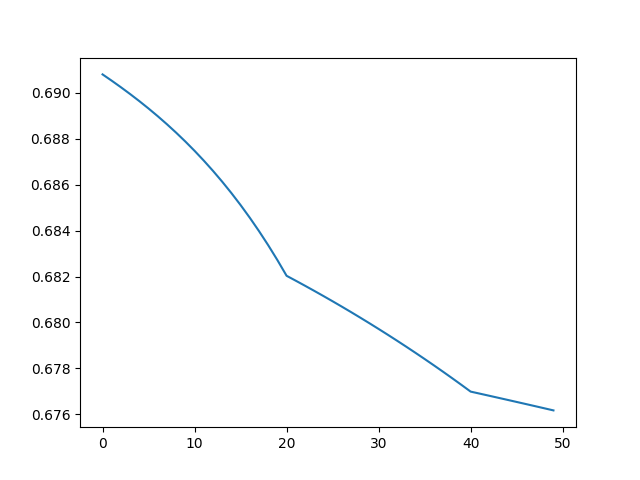
\includegraphics[scale=0.5]{train_loss_q3}
\end{wrapfigure}\\
Testing Accuracy: 100\%\\
The figure is shown at right hand side\newpage
\textbf{4a)}\\
$W_{1} = \begin{bmatrix}-0.1698 & 0.2748 & 0.2536\\
0.0057 & 0.0080 & 0.0358\\\end{bmatrix}\\ W_{2} =
\begin{bmatrix}
1.0186 & -0.2970 & 0.9568\\
-0.0795 & 1.0447 & 1.0025\\
-0.4609 & 0.4832 & 0.3152\\\end{bmatrix}$ \\      
Test Accuracy: 93.6 \%\\
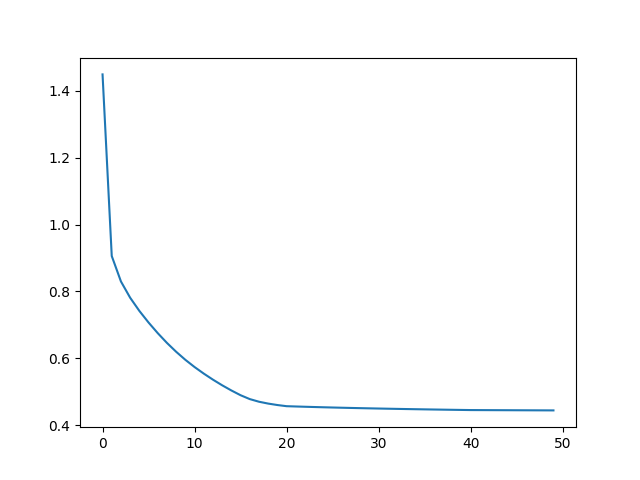
\includegraphics[scale=0.5]{train_loss_q4a}\\
\textbf{4b)}\\
For learning rate = 0.01,\\
$ W_{1} = \begin{bmatrix}
0.8627 & -0.0390 &  0.8312\\
-2.0662 & -1.3738 & -0.3055\end{bmatrix}\\, W_{2} = 
\begin{bmatrix}
1.4603 & -0.8739 & -0.7407\\
-0.1039 & 0.9317 & 0.6105\\
-0.3664 & 0.5522 & 0.7302\end{bmatrix}$ \\     
Testing Accuracy: 54.9 \%\\
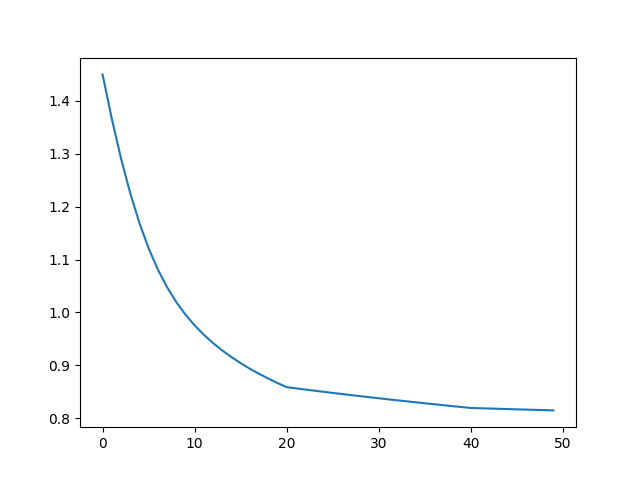
\includegraphics[scale=0.5]{train_loss_q4b1}\newpage
For learning rate = 0.1,\\
$W_{1} = \begin{bmatrix}-0.1698 & 0.2748 & 0.2536\\
0.0057 & 0.0080 & 0.0358\\\end{bmatrix}\\ W_{2} =
\begin{bmatrix}
1.0186 & -0.2970 & 0.9568\\
-0.0795 & 1.0447 & 1.0025\\
-0.4609 & 0.4832 & 0.3152\\\end{bmatrix}$ \\      
Testing Accuracy: 93.6 \%\\
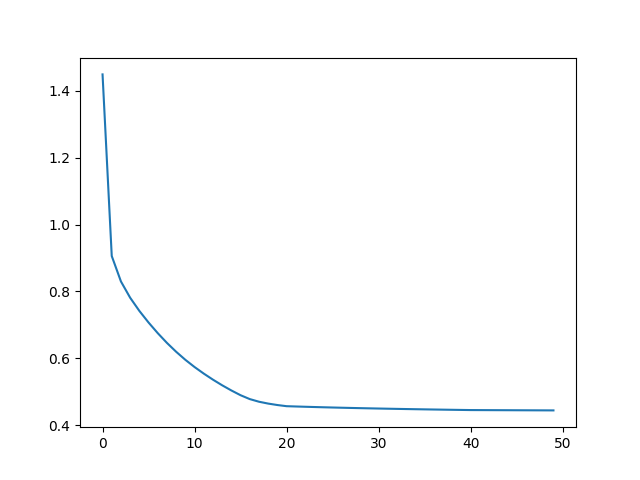
\includegraphics[scale=0.5]{train_loss_q4a}\\
For learning rate = 1,\\
$W_{1} = \begin{bmatrix}
0.2537 & -0.4833 & -0.3027\\
-3.1115 & -1.5151 & -0.7082
\end{bmatrix}, W_{2} = \begin{bmatrix}
1.5082 & -0.6465 & -0.1343\\
0.4220 & 0.9842 & 1.1584\\
-0.9402 &  0.2722 & -0.4241
\end{bmatrix}$\\        
Testing Accuracy: 50.25 \%\\
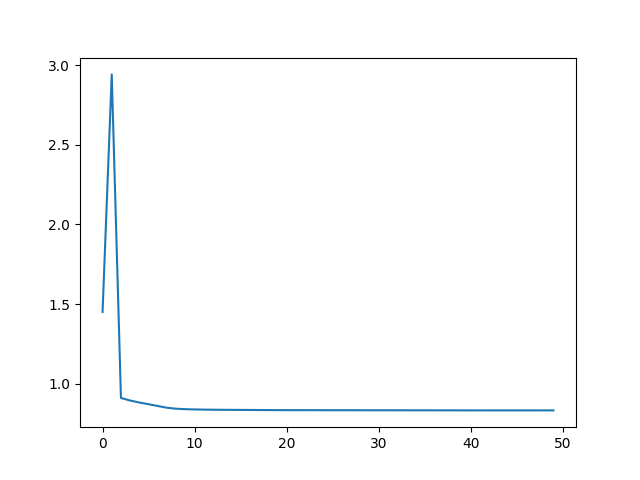
\includegraphics[scale=0.5]{train_loss_q4b2}\\[0.2in]
From these 3 results, we can find out that 0.1 learning rate gives the best testing accuracy among 3 different learning rate values. Therefore, either too high or too low learning rate will not increase the testing accuracy, but an appropriate value will. (Too high will lead to loss explode and too low will make the weights update too slow!)\newpage
\textbf{4c)}\\
In the following test, I will run the following 100 times to get a optimal learning rate for the question:\\
\indent Each time I will set $W_{1},W_{2}$ into some random value, and then I will find the optimal learning rate range from (0.05 to 0.5) that gives the highest test accuracy for that random case.\\[0.2in]
Finally, I get a mean value for these 100 cases: 0.21845\\
Then I will put it into the test set, \\[0.4in]
Use the weight given in (a), testing accuracy: 93.55\% (See figure below)\\ 
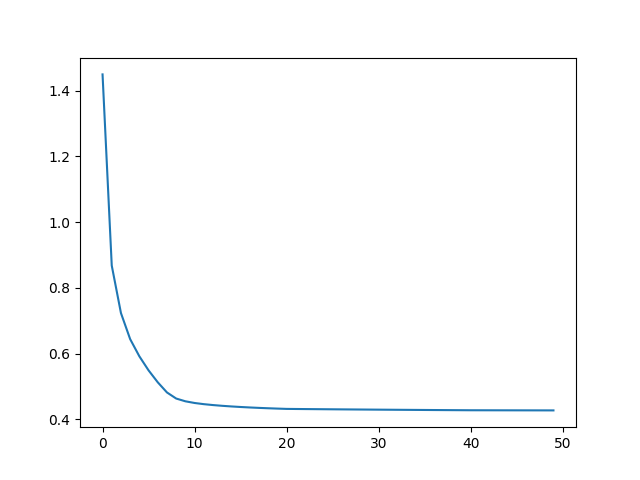
\includegraphics[scale=0.5]{train_loss_q4c1}\\[0.4in]
A random weight, testing accuracy: 72.95\% (See figure below)\\
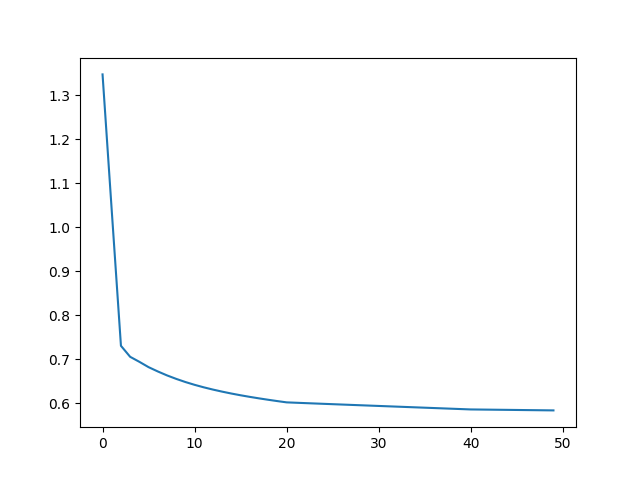
\includegraphics[scale=0.5]{train_loss_q4c2}\\[0.4in]
(10 random weights, average testing accuracy: 66.86\%) \\
\end{document}
